\section{A common use-case}
\subsection{Retry my results}
\begin{frame}
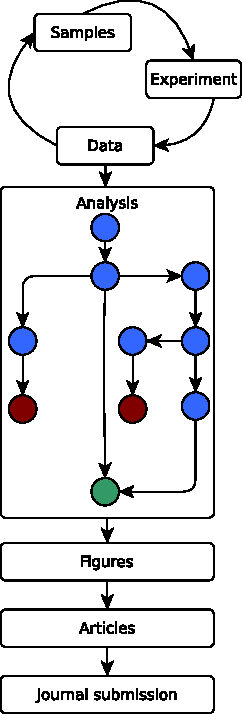
\includegraphics[width=0.1\textwidth]{images/schema_soumission_fair.pdf}
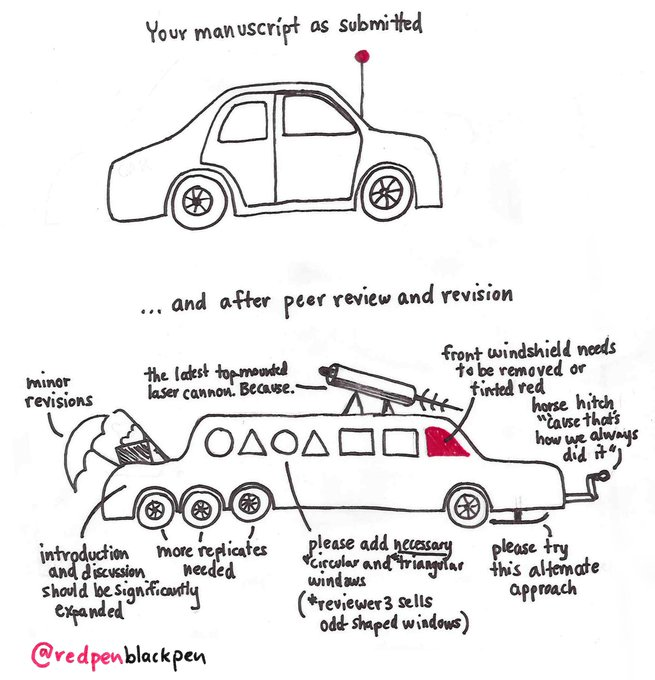
\includegraphics[width=0.1\textwidth]{images/review.jpg}
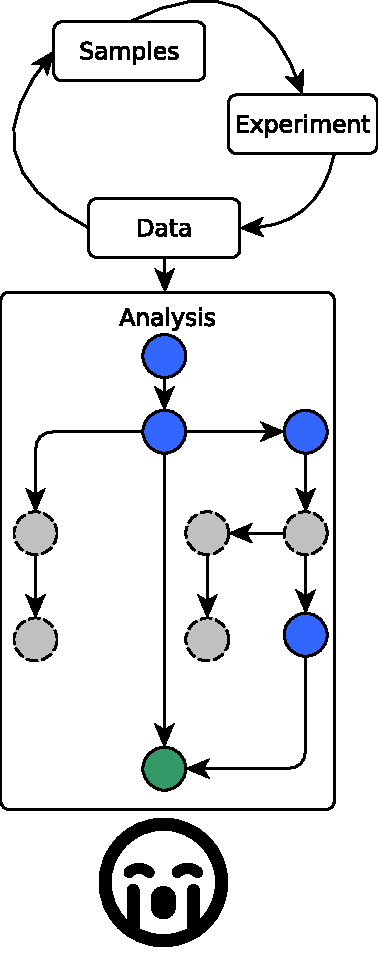
\includegraphics[width=0.1\textwidth]{images/schema_soumission_fair_echec.pdf}
\centering{What are the changes ?}
\begin{columns}
\column{.5\textwidth}
\begin{itemize}
	\item Tool version
	\item Packages
	\item Environment variables
\end{itemize}
\column{.5\textwidth}
\begin{itemize}
	\item OS version
	\item The computer 
	\item ...
\end{itemize}
\end{columns}
\end{frame}

\subsection{The use of packaging}
\begin{frame}{Encapsulation levels}
\emph{Encapsulation: capture the system environment of applications (OS, packages,libraries) to control their execution}
\begin{itemize}
	\item Hardware virtualisation (virtual machines) 
\includegraphics[width=0.1\textwidth]{images/VM_logo.png} 
	\item OS virtualisation (images and containers) 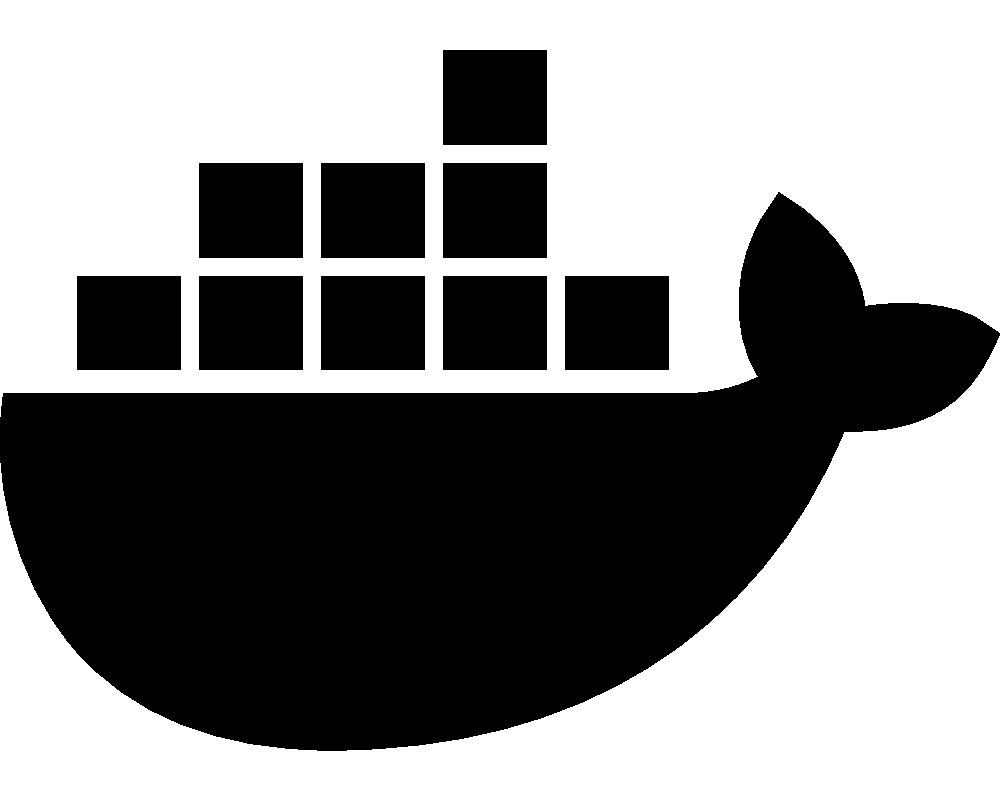
\includegraphics[width=0.1\textwidth]{images/docker.pdf} 
\includegraphics[width=0.1\textwidth]{images/singularity_logo.pdf} 
	\item Environment management (package manager) 
\includegraphics[width=0.1\textwidth]{images/conda_logo.pdf} 
\end{itemize}
\end{frame}
\subsection{Example with R}
\begin{frame}{Example of R and package installation}{Classical installation}
\begin{itemize}
	\item Start with a computer and a specific OS
	\item Inside, we installed a new 
\includegraphics[width=0.1\textwidth]{images/r-project.pdf} application
	\item 
\includegraphics[width=0.1\textwidth]{images/r-project.pdf} need some dependencies
	\item we tested the last R version --> might be conflicts
\end{itemize}

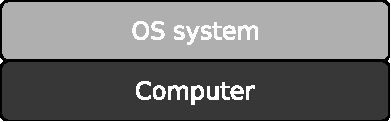
\includegraphics[width=0.1\textwidth]{images/conda_env_1.pdf} 
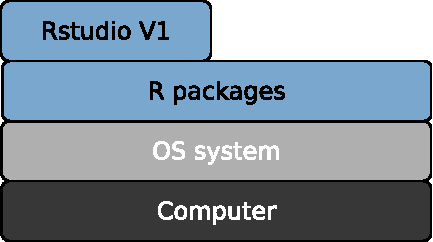
\includegraphics[width=0.1\textwidth]{images/conda_env_2.pdf} 
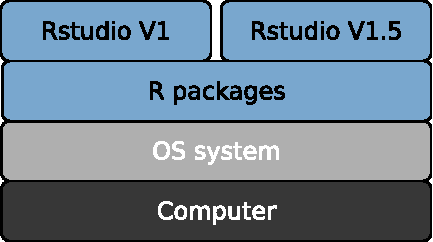
\includegraphics[width=0.1\textwidth]{images/conda_env_3.pdf} 
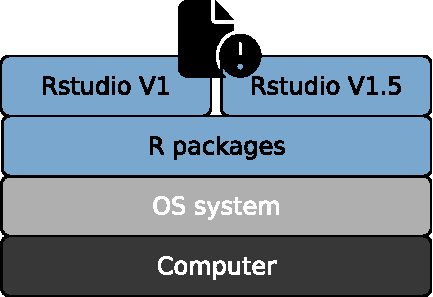
\includegraphics[width=0.1\textwidth]{images/conda_env_4.pdf} 
\end{frame}

\begin{frame}
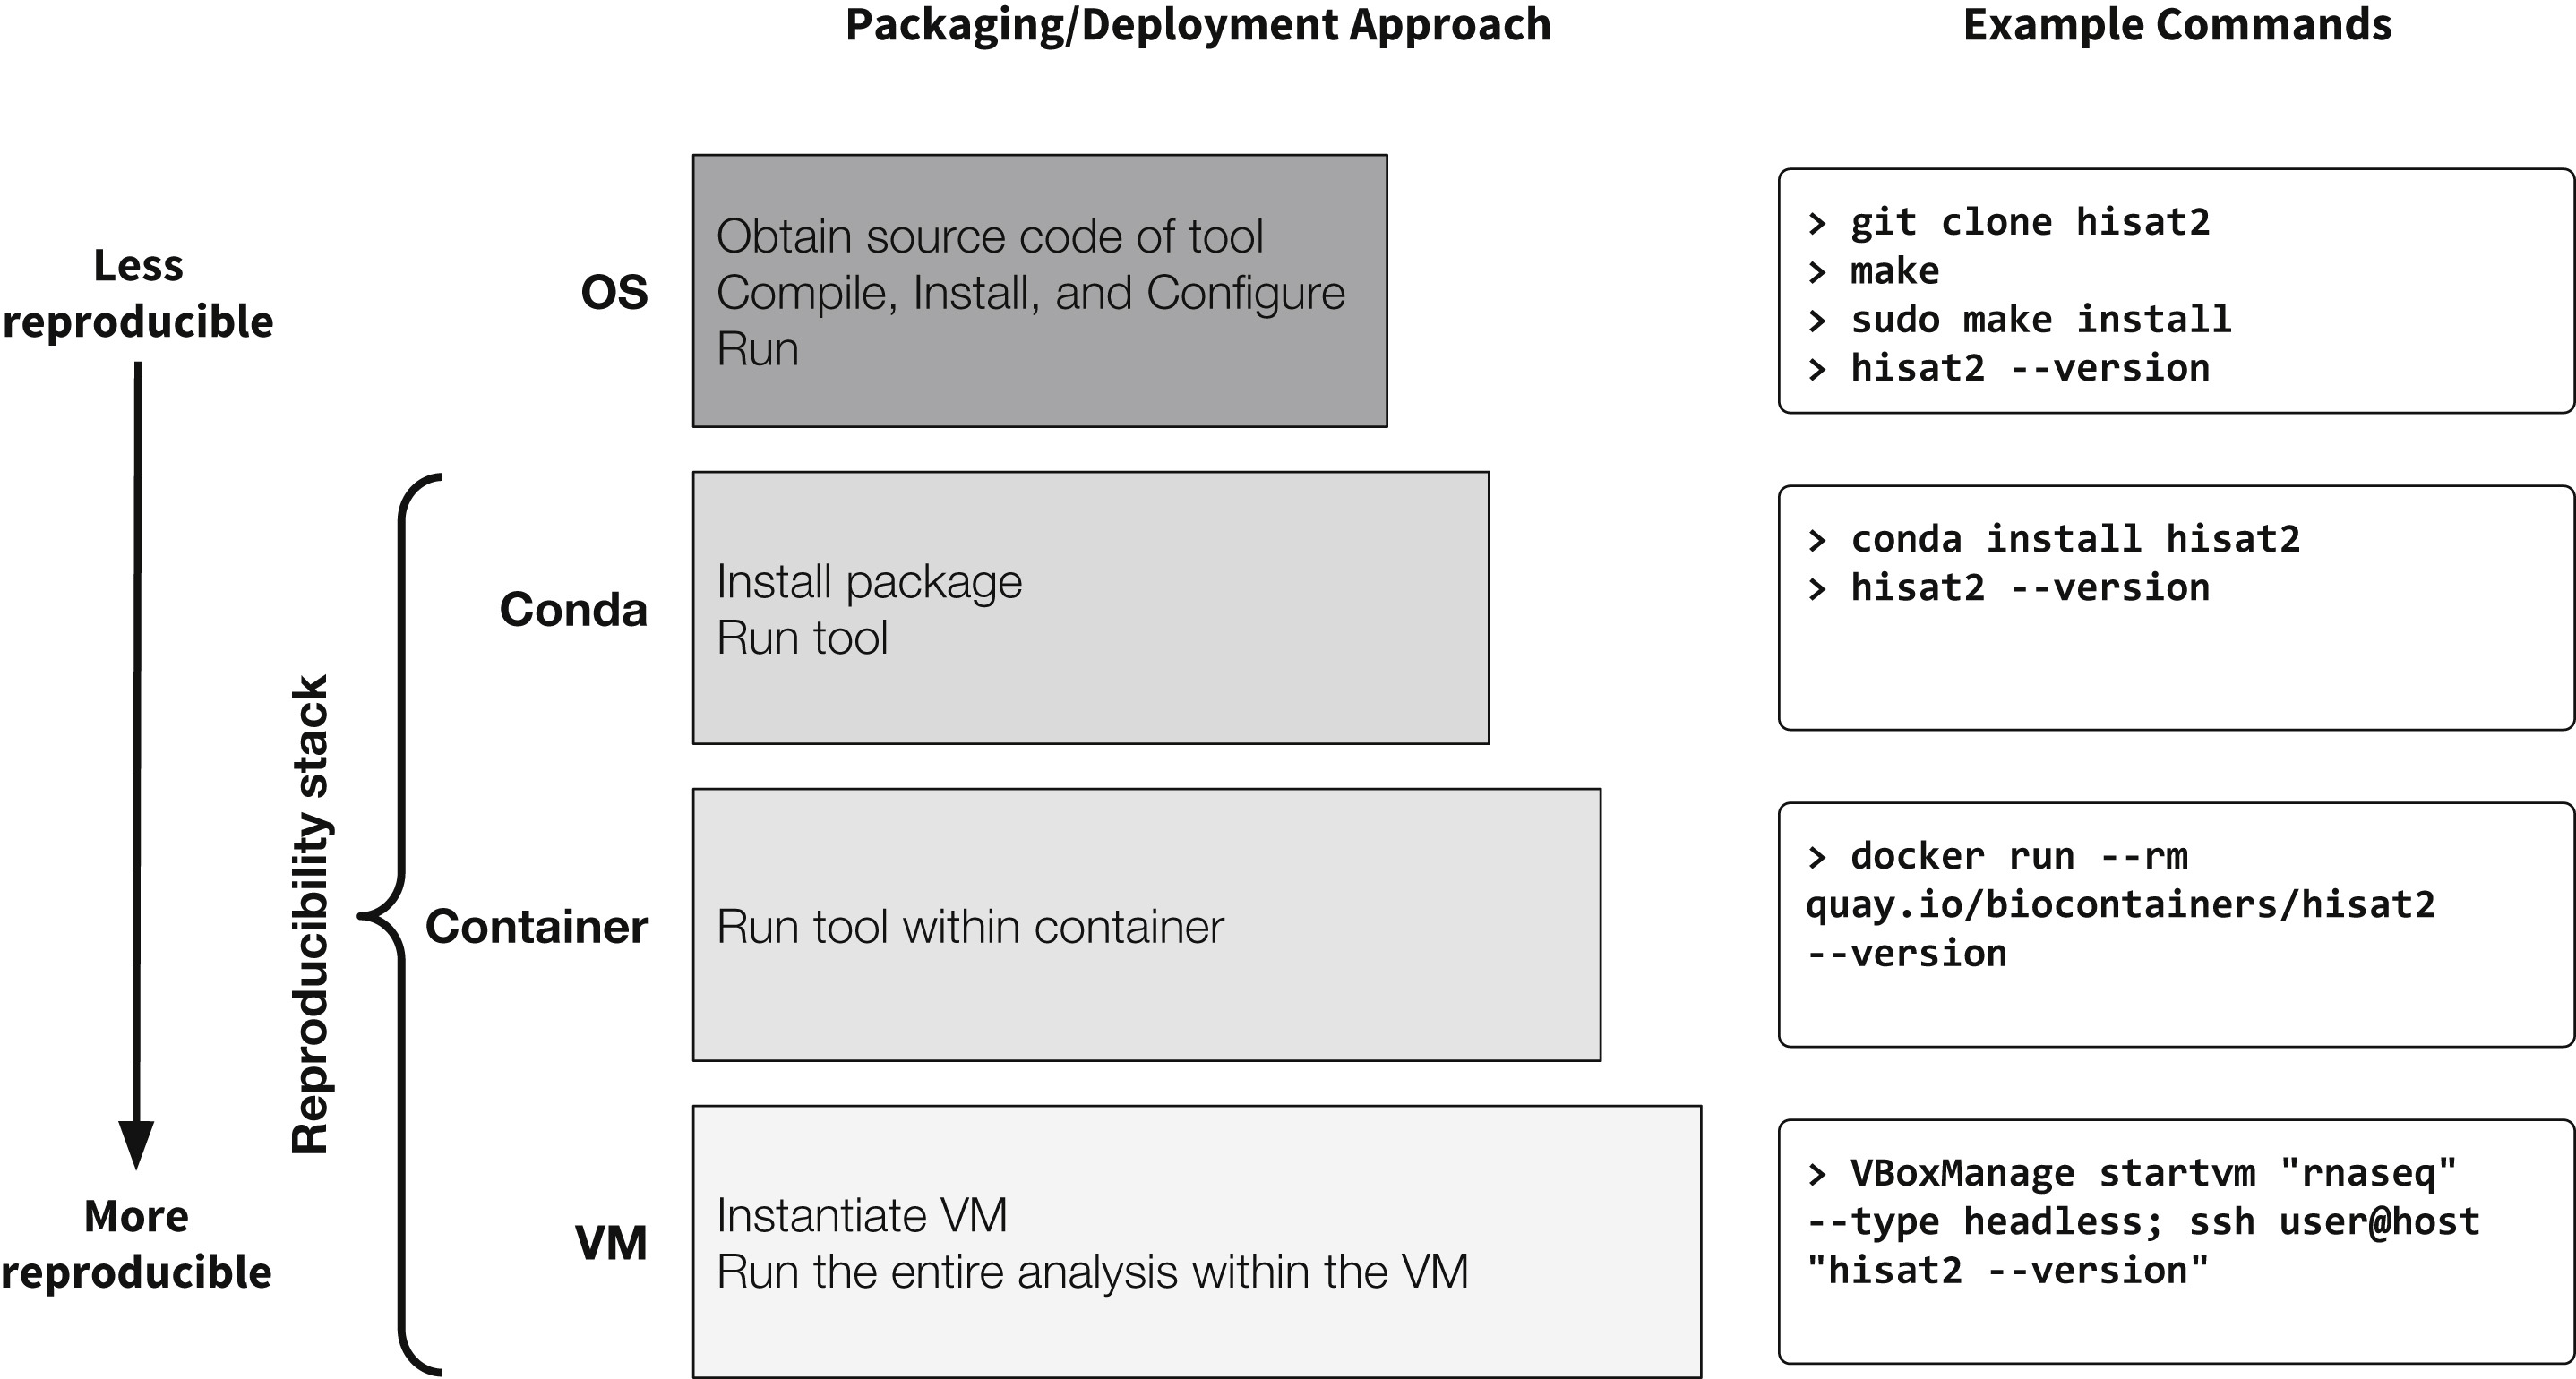
\includegraphics[width=0.1\textwidth]{images/reproductibility.jpg} \footnote{Practical Computational Reproducibility in the Life Sciences
Grüning et al, Cell Systems, 2018. DOI 10.1016/j.cels.2018.03.014}

\end{frame}
%% A METTRE EN FIN DE DIAPO
\begin{frame}

    A package first
    One tool, one container
    Tool and container versions should be explicit
    Avoid using ENTRYPOINT
    Reduce the size of your container as much as possible
    Keep data outside of the container
    Add functional testing logic
    Check the license of the software
    Make your package or container discoverable
    Provide reproducible and documented builds
    Provide helpful usage message

\end{frame}